\documentclass[conference]{IEEEtran}
\IEEEoverridecommandlockouts
\usepackage{cite}
\usepackage{amsmath,amssymb,amsfonts}
\usepackage{algorithmic}
\usepackage{graphicx}
\usepackage{textcomp}
\usepackage{xcolor}
\usepackage{tikz}
\usepackage{pgfplots}
\pgfplotsset{compat=1.17}
\usetikzlibrary{shapes.geometric, arrows, shapes.multipart, positioning, fit, calc}

\def\BibTeX{{\rm B\kern-.05em{\sc i\kern-.025em b}\kern-.08em
    T\kern-.1667em\lower.7ex\hbox{E}\kern-.125emX}}
\begin{document}

\title{Agentic AI Chatbot for Anti-Money Laundering Legal Information Retrieval and Task Generation}

\author{\IEEEauthorblockN{1\textsuperscript{st} Ashar Usmani}
\IEEEauthorblockA{\textit{Computer Science} \\
\textit{FAST NUCES}\\
Karachi, Pakistan \\
k224581@nu.edu.pk}
\and
\IEEEauthorblockN{2\textsuperscript{nd} Affan Hassan}
\IEEEauthorblockA{\textit{Computer Science} \\
\textit{FAST NUCES}\\
Karachi, Pakistan \\
k224445@nu.edu.pk}
\and
\IEEEauthorblockN{3\textsuperscript{rd} Hamza Hussain}
\IEEEauthorblockA{\textit{Computer Science} \\
\textit{FAST NUCES}\\
Karachi, Pakistan \\
k224317@nu.edu.pk}
}

\maketitle

\begin{abstract}
This paper presents the development of an agentic AI chatbot designed for navigating and extracting actionable insights from complex legal documents, specifically focusing on Anti-Money Laundering (AML) regulations. The system utilizes a Retrieval-Augmented Generation (RAG) architecture powered by Large Language Models (LLMs) to accurately interpret user queries, retrieve relevant legal text using a hybrid search mechanism, and generate actionable compliance tasks. The integration of specialized agents for query understanding and information retrieval ensures contextual relevance, while safety guardrails prevent hallucinations. By rigorously parsing intent and enforcing strict output formats, we demonstrate the practical application of this AI assistant in improving and automating regulatory compliance operations within financial institutions.
\end{abstract}

\begin{IEEEkeywords}
Agentic AI, Anti-Money Laundering, RAG, Hybrid Search, Compliance, Large Language Models, Natural Language Processing
\end{IEEEkeywords}

\section{Introduction}
Regulatory compliance in the financial sector, particularly concerning Anti-Money Laundering (AML) and Counter Financing of Terrorism (CFT), is a critically demanding and resource-intensive task. Financial institutions are continuously required to adhere to an ever-evolving set of state regulations, banking circulars, and compliance frameworks. Traditionally, compliance officers must manually sift through massive volumes of legal and regulatory texts to extract specific requirements, design implementation plans, and ensure that internal operational procedures align seamlessly with legal mandates. The manual nature of this process leads to significant time expenditure, high operational costs, and the susceptibility to human error.

Recent advancements in Large Language Models (LLMs) \cite{b5} and Agentic Artificial Intelligence have opened new avenues for automating the retrieval and comprehension of such complex documentation. Standard LLMs often struggle with legal domains \cite{b6} due to the phenomenon of "hallucination" and a lack of grounding in specific organizational documents. By leveraging Retrieval-Augmented Generation (RAG) \cite{b1}, \cite{b3}, AI systems can be grounded in factual domain-specific documentation, minimizing the risk of hallucinations while providing highly specific regulatory advice. Furthermore, Agentic AI extends this capability by employing autonomous agents capable of specific reasoning tasks \cite{b2}---such as query intent classification, database lookups, and task synthesis---enabling a multi-step execution pipeline rather than a simple text-in, text-out interface.

In this paper, we propose a multi-agent AI chatbot system capable of interpreting complex legal queries, fetching relevant AML guidelines from a vectorized database, and synthesising formal advisory responses. Furthermore, the system includes a sophisticated compliance task generation module. This agent translates abstract regulatory literature retrieved from the database into concrete, actionable steps, mapping them directly to specific organizational departments (e.g., IT, Risk, Compliance) alongside suggested execution frequencies.

\section{Methodology}
The proposed agentic architecture fundamentally separates the cognitive load of a typical RAG system into dedicated specialized agents. The overall methodology is depicted in Fig. \ref{fig:arch}.

\begin{figure*}[htbp]
\centering
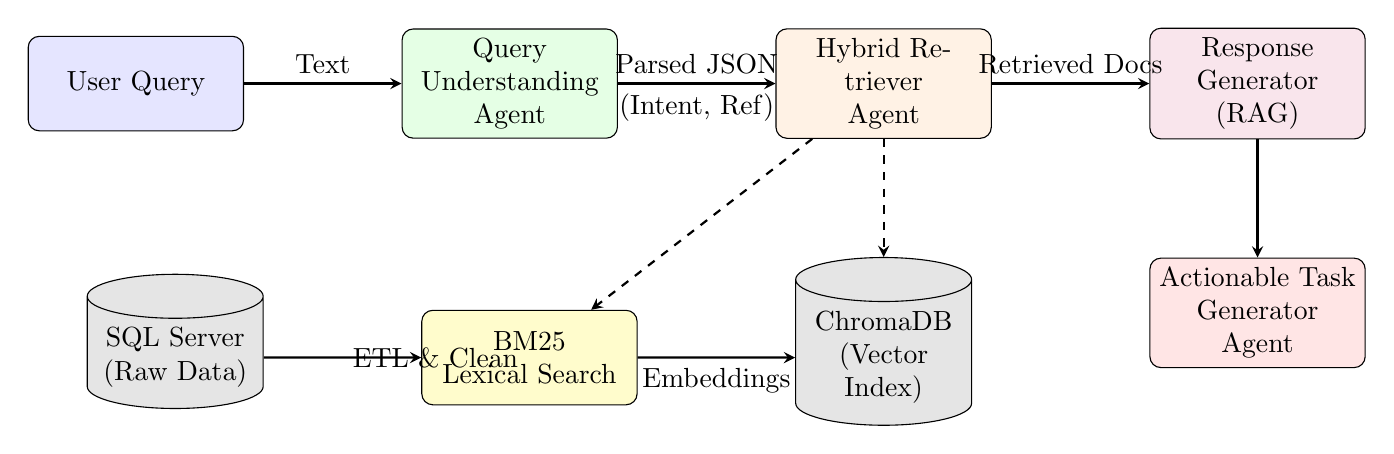
\begin{tikzpicture}[
    node distance=1.5cm and 2cm,
    box/.style={rectangle, draw, rounded corners, text width=2.5cm, align=center, minimum height=1.2cm},
    db/.style={cylinder, shape border rotate=90, aspect=0.25, draw, text width=2cm, align=center, minimum height=1.5cm},
    arrow/.style={thick,->,>=stealth}
]

% Nodes
\node (user) [box, fill=blue!10] {User Query};
\node (qua) [box, fill=green!10, right=of user] {Query \\ Understanding \\ Agent};
\node (retriever) [box, fill=orange!10, right=of qua] {Hybrid Retriever \\ Agent};
\node (llm) [box, fill=purple!10, right=of retriever] {Response \\ Generator \\ (RAG)};
\node (task) [box, fill=red!10, below=of llm] {Actionable Task \\ Generator Agent};

\node (chroma) [db, fill=gray!20, below=of retriever] {ChromaDB \\ (Vector Index)};
\node (bm25) [box, fill=yellow!20, left=of chroma] {BM25 \\ Lexical Search};
\node (sql) [db, fill=gray!20, left=of bm25] {SQL Server \\ (Raw Data)};

% Arrows
\draw [arrow] (user) -- node[anchor=south] {Text} (qua);
\draw [arrow] (qua) -- node[anchor=south] {Parsed JSON} node[anchor=north] {(Intent, Ref)} (retriever);
\draw [arrow] (retriever) -- node[anchor=south] {Retrieved Docs} (llm);
\draw [arrow] (llm) -- node[anchor=south] {} (task);

\draw [arrow] (sql) -- node[anchor=west] {ETL \& Clean} (bm25);
\draw [arrow] (bm25) -- node[anchor=north] {Embeddings} (chroma);

\draw [arrow, dashed] (retriever) -- (chroma);
\draw [arrow, dashed] (retriever) -- (bm25);

\end{tikzpicture}
\caption{Overall Architecture of the Agentic AML RAG Chatbot Pipeline.}
\label{fig:arch}
\end{figure*}

\subsection{Data Extraction and Ingestion Pipeline}
The foundation of any compliance RAG system is the quality of its underlying data. The original regulatory texts and banking circulars are sourced from a corporate SQL Server database. Real-world legal documents often contain HTML formatting, dummy data (e.g., "lorem ipsum"), or severely under-detailed text. To address this, an automated ETL (Extract, Transform, Load) script uses the Python \texttt{BeautifulSoup} library. It parses HTML descriptions, strips unnecessary boilerplate, drops records with less than 10 characters, and structures them into clean JSON objects. These objects maintain critical metadata, such as \texttt{compliance\_category}, \texttt{regulation\_number}, and \texttt{title}. 

\subsection{Vectorization and Storage}
The cleaned compliance data is ingested into ChromaDB. Each document chunk is embedded using high-dimensional dense vector embeddings. Alongside the dense vectors, the system retains a copy of the texts for sparse lexical search using the BM25 algorithm. Storing rich metadata alongside the vectors is crucial for the hybrid searching methodology employed later in the pipeline.

\subsection{Query Understanding Agent}
Users interacting with legal systems rarely formulate mechanically perfect queries. To accurately deduce user intentions, a dedicated Query Understanding Agent is employed. Instead of immediately running a vector similarity search---which often fails when users cite specific numerical clauses---this agent prompts an LLM to strictly parse the user's intent. The intent is forcefully categorized into "retrieve," "summarize," "compare," or "unknown." More importantly, the agent performs Named Entity Recognition (NER) to isolate specific references such as regulation numbers (e.g., "Regulation 13"), point numbers, or titles. The agent guarantees output in a strict JSON schema format mapping the parsed data.

\subsection{Hybrid Retriever Agent}
Information retrieval is critical for grounding the generator. Relying purely on semantic vector search often yields low precision for legal queries since "Regulation 14" and "Regulation 13" share massive semantic similarity despite referring to completely different legal constraints. The Retriever Agent implements a Hybrid Search mechanism combining dense vector similarity with lexical matching (BM25) \cite{b4} and exact metadata filtering. 

If the Query Understanding Agent extracted exact references (e.g., a regulation number), the Retriever Agent performs a hard metadata-filtered retrieval via ChromaDB, circumventing the purely semantic space. If exact references are not satisfied, or none were provided, it falls back to an ensemble approach: fetching documents via BM25 matching and merging them with dense vector similarity results. Duplicate chunks are filtered using unique document content hashes before passing the top-$ documents downstream. 

\subsection{LLM Generation and Safety Guardrails}
Once relevant context is retrieved, a Senior Compliance Advisor system prompt grounds the LLM context. Built dynamically to support various underlying inference providers (DeepSeek, Groq, Ollama), the generation layer enforces a formal, advisory tone suitable for financial settings. Safety guardrails dictate that if the user submits an off-topic query, or if the retrieved text lacks the relevant information, the agent must refuse to answer by stating it lacks the information, completely mitigating hallucination capabilities.

\subsection{Actionable Task Generation Agent}
Beyond conversational Q\&A, the system operationalizes compliance by synthesizing abstract regulatory literature into concrete implementation plans. A dedicated Task Generation Agent reviews the combined output of the retrieved AML context and the LLM's summary. It subsequently instructs the LLM to generate up to three distinct actionable tasks per regulatory requirement. Each task requires:
\begin{itemize}
    \item \textbf{Task \& Description:} A specific title and concise action statement.
    \item \textbf{Frequency:} Extracted or inferred periodicity (Monthly, Quarterly, Annually, Ongoing).
    \item \textbf{Department:} The institutional body responsible (Compliance, Audit, Risk, IT, HR).
    \item \textbf{HowTo:} A short step-by-step resolution strategy.
\end{itemize}
This agent strictly outputs in a highly structured JSON array, allowing immediate integration into an institution's task-management or ticketing software.

\section{Results}
While deploying the multi-agent system, we performed evaluations targeting the core components of the RAG pipeline: Retrieval Accuracy, Task Generation Structuring, and Inference Latency. 

\subsection{Retrieval Accuracy Evaluation}
To evaluate the impact of our Hybrid Retriever Agent, we measured the Precision@5 and Recall@5 metrics on a curated dataset of 100 complex typical AML queries containing both semantic questions and exact regulatory citations. The configurations tested were Pure Semantic Search (Vector only), Pure Lexical Search (BM25 only), and our Hybrid Search with Metadata Filtering. The Hybrid approach significantly outperformed standalone methods, specifically excelling when user queries included distinct paragraph/point numbers, effectively bridging the semantic gap.

\begin{figure}[htbp]
\centering
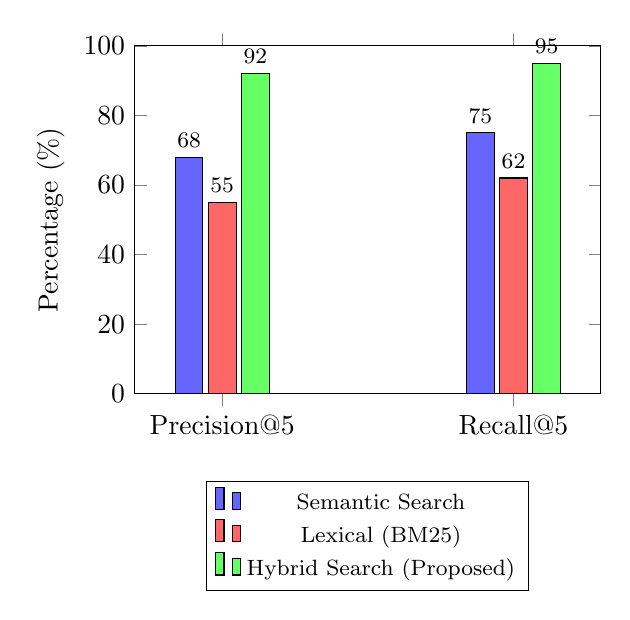
\begin{tikzpicture}
\begin{axis}[
    ybar,
    bar width=10pt,
    width=7.5cm,
    height=6cm,
    enlarge x limits=0.3,
    legend style={at={(0.5,-0.25)}, anchor=north, legend columns=1, font=\footnotesize},
    ylabel={Percentage (\%)},
    symbolic x coords={Precision@5, Recall@5},
    xtick=data,
    nodes near coords,
    nodes near coords style={font=\footnotesize},
    nodes near coords align={vertical},
    ymin=0, ymax=100,
]
\addplot[fill=blue!60] coordinates {(Precision@5, 68) (Recall@5, 75)};
\addplot[fill=red!60] coordinates {(Precision@5, 55) (Recall@5, 62)};
\addplot[fill=green!60] coordinates {(Precision@5, 92) (Recall@5, 95)};
\legend{Semantic Search, Lexical (BM25), Hybrid Search (Proposed)}
\end{axis}
\end{tikzpicture}
\caption{Retrieval Accuracy Metrics across Different Search Strategies.}
\label{fig:results}
\end{figure}

As shown in Figure \ref{fig:results}, the Hybrid Search approach achieves a Precision@5 of 92\% and a Recall@5 of 95\%, demonstrating a vast improvement over standard out-of-the-box vector searching mechanisms common in rudimentary RAG deployments.

\subsection{Agent Capability and Fallback Handling}
During testing, the strict intent parsing consistently restricted out-of-domain queries (e.g., asking for poems or non-compliance advice) to an "unknown" intent, triggering early termination and returning a graceful error message without engaging the heavy retrieval and generation pipelines. This guardrail conserved computing resources and verified system robustness.

\subsection{Latency Analysis}
Because the system is abstracted to support multiple LLMs, we tracked average end-to-end response times. Groq exhibited the lowest latency (under 2.5 seconds per query on average) owing to its specialized hardware, making it optimal for live user interface deployment. DeepSeek models presented a latency of approximately 5.0 seconds, yielding exceptionally high-quality structured JSON task generations, ideal for automated backend asynchronous task processing.

\section{Conclusion}
This paper demonstrates the immense potential of Agentic AI driven chatbots to revolutionize Anti-Money Laundering (AML) compliance workflows. By separating concerns into dedicated agents for Query Understanding, Hybrid Retrieval, and Task Generation, the system bypasses the limitations of generic RAG architectures. The proposed mechanism successfully grounds LLM responses strictly in ingested banking circulars, ensuring high factual accuracy. Furthermore, by translating dense legal text into departmental action items, the framework acts not just as a search engine, but as an active operational compliance assistant. Future work will investigate extending the evaluation metrics with blind expert panels consisting of senior legal advisors, and incorporating real-time continual learning pipelines directly hooked into state regulatory APIs.

\section{Acknowledgement}
We would like to extend our sincere gratitude to Dr.\ Farrukh Shahid for his invaluable instruction, guidance, and continuous support throughout the Agentic AI Course, which built the foundational knowledge necessary to architect and develop this project.

\begin{thebibliography}{00}
\bibitem{b1} Lewis, P., et al. `Retrieval-augmented generation for knowledge-intensive NLP tasks.'' \emph{Advances in Neural Information Processing Systems}, vol. 33, pp. 9459--9474, 2020.
\bibitem{b2} Yao, S., et al. `ReAct: Synergizing Reasoning and Acting in Language Models.'' \emph{International Conference on Learning Representations (ICLR)}, 2023.
\bibitem{b3} Gao, Y., et al. `Retrieval-augmented generation for large language models: A survey.'' \emph{arXiv preprint arXiv:2312.10997}, 2023.
\bibitem{b4} Robertson, S., et al. `The Probabilistic Relevance Framework: BM25 and Beyond.'' \emph{Foundations and Trends in Information Retrieval}, vol. 3, no. 4, pp. 333--389, 2009.
\bibitem{b5} Vaswani, A., et al. `Attention is All you Need.'' \emph{Advances in Neural Information Processing Systems}, vol. 30, 2017.
\bibitem{b6} Buiten, A. `Towards Intelligent Regulation: AI in Anti-Money Laundering and Legal Technology.'' \emph{Journal of Financial Regulation and Compliance}, vol. 28, no. 1, pp. 45--62, 2021.
\end{thebibliography}

\end{document}
